\chapter{Flujos y cortes}

En este cap\'itulo, nos concentraremos
en los dos problemas siguientes:

\begin{itemize}
	\item \key{Encontrar un flujo m\'aximo}:
	Cu\'al es la mayor cantidad de flujo que se puede
	enviar desde un nodo a otro nodo?
	\item \key{Encontrar un corte m\'inimo}:
	Cu\'al es el conjunto de aristas de menor peso
	que separa a dos nodos del grafo?
\end{itemize}

La entrada para ambos problemas es un grafo
dirigido y pesado que contiene dos nodos especiales:
La \key{fuente} es un nodo sin aristas entrantes,
y el \key{sumidero} es un nodo sin aristas salientes.

Tomemos el siguiente grafo como ejemplo
donde el nodo 1 es la fuente y el nodo 6
es el sumidero:

\begin{center}
	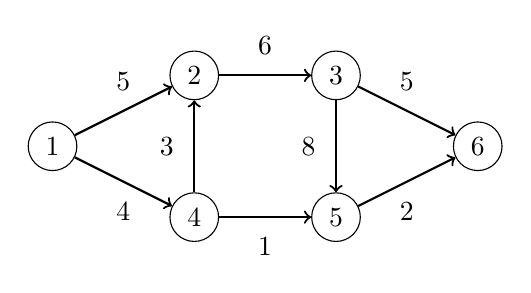
\begin{tikzpicture}[scale=0.9]
	\node[draw, circle] (1) at (1,2) {$1$};
	\node[draw, circle] (2) at (3,3) {$2$};
	\node[draw, circle] (3) at (5,3) {$3$};
	\node[draw, circle] (4) at (7,2) {$6$};
	\node[draw, circle] (5) at (3,1) {$4$};
	\node[draw, circle] (6) at (5,1) {$5$};
	\path[draw,thick,->] (1) -- node[font=\small,label=5] {} (2);
	\path[draw,thick,->] (2) -- node[font=\small,label=6] {} (3);
	\path[draw,thick,->] (3) -- node[font=\small,label=5] {} (4);
	\path[draw,thick,->] (1) -- node[font=\small,label=below:4] {} (5);
	\path[draw,thick,->] (5) -- node[font=\small,label=below:1] {} (6);
	\path[draw,thick,->] (6) -- node[font=\small,label=below:2] {} (4);
	\path[draw,thick,<-] (2) -- node[font=\small,label=left:3] {} (5);
	\path[draw,thick,->] (3) -- node[font=\small,label=left:8] {} (6);
	\end{tikzpicture}
\end{center}

\subsubsection{Flujo m\'aximo}

\index{flujo}
\index{flujo m\'aximo}

En el problema del \key{flujo m\'aximo},
nuestro objetivo es enviar tanto flujo como sea
posible desde la fuente hacia el sumidero.
El peso de cada arista es una capacidad
que restringe el flujo
que puede pasar por la arista.
En cada nodo intermedio,
el flujo que entra y el flujo
que sale tienen que ser iguales.

Por ejemplo, el flujo m\'aximo
en el grafo de ejemplo es 7.
La siguiente imagen nos muestra
como podemos encontrar la ruta del flujo:

\begin{center}
	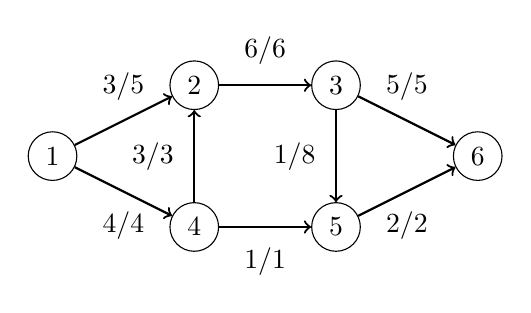
\begin{tikzpicture}[scale=0.9]
	\node[draw, circle] (1) at (1,2) {$1$};
	\node[draw, circle] (2) at (3,3) {$2$};
	\node[draw, circle] (3) at (5,3) {$3$};
	\node[draw, circle] (4) at (7,2) {$6$};
	\node[draw, circle] (5) at (3,1) {$4$};
	\node[draw, circle] (6) at (5,1) {$5$};
	\path[draw,thick,->] (1) -- node[font=\small,label=3/5] {} (2);
	\path[draw,thick,->] (2) -- node[font=\small,label=6/6] {} (3);
	\path[draw,thick,->] (3) -- node[font=\small,label=5/5] {} (4);
	\path[draw,thick,->] (1) -- node[font=\small,label=below:4/4] {} (5);
	\path[draw,thick,->] (5) -- node[font=\small,label=below:1/1] {} (6);
	\path[draw,thick,->] (6) -- node[font=\small,label=below:2/2] {} (4);
	\path[draw,thick,<-] (2) -- node[font=\small,label=left:3/3] {} (5);
	\path[draw,thick,->] (3) -- node[font=\small,label=left:1/8] {} (6);
	\end{tikzpicture}
\end{center}

La notaci\'on $v/k$ significa
que un flujo de $v$ unidades atraviesa
una arista con capacidad de $k$ unidades.
El tama\~no del flujo es $7$,
ya que la fuente env\'ia $3+4$ unidades de flujo
y el sumidero recibe $5+2$ unidades de flujo.
Se puede ver f\'acilmente que el flujo es m\'aximo,
porque la capacidad total de las aristas
que van dirigidas al sumidero es $7$.

\subsubsection{Corte M\'inimo}

\index{corte}
\index{corte m\'inimo}

En el problema del \key{corte m\'inimo},
el objetivo es eliminar un conjunto
de aristas del grafo
de tal forma que no exista un camino
desde la fuente hacia el sumidero
y que el peso total de las aristas
eliminadas sea m\'inimo.

El tama\~no del corte m\'inimo en el grafo de ejemplo es 7.
Basta con eliminar las aristas $2 \rightarrow 3$
y $4 \rightarrow 5$:

\begin{center}
	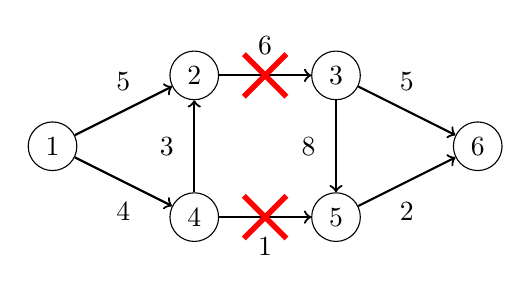
\begin{tikzpicture}[scale=0.9]
	\node[draw, circle] (1) at (1,2) {$1$};
	\node[draw, circle] (2) at (3,3) {$2$};
	\node[draw, circle] (3) at (5,3) {$3$};
	\node[draw, circle] (4) at (7,2) {$6$};
	\node[draw, circle] (5) at (3,1) {$4$};
	\node[draw, circle] (6) at (5,1) {$5$};
	\path[draw,thick,->] (1) -- node[font=\small,label=5] {} (2);
	\path[draw,thick,->] (2) -- node[font=\small,label=6] {} (3);
	\path[draw,thick,->] (3) -- node[font=\small,label=5] {} (4);
	\path[draw,thick,->] (1) -- node[font=\small,label=below:4] {} (5);
	\path[draw,thick,->] (5) -- node[font=\small,label=below:1] {} (6);
	\path[draw,thick,->] (6) -- node[font=\small,label=below:2] {} (4);
	\path[draw,thick,<-] (2) -- node[font=\small,label=left:3] {} (5);
	\path[draw,thick,->] (3) -- node[font=\small,label=left:8] {} (6);

	\path[draw=red,thick,-,line width=2pt] (4-.3,3-.3) -- (4+.3,3+.3);
	\path[draw=red,thick,-,line width=2pt] (4-.3,3+.3) -- (4+.3,3-.3);
	\path[draw=red,thick,-,line width=2pt] (4-.3,1-.3) -- (4+.3,1+.3);
	\path[draw=red,thick,-,line width=2pt] (4-.3,1+.3) -- (4+.3,1-.3);
	\end{tikzpicture}
\end{center}

Despu\'es de eliminar las aristas,
no hay ning\'un camino desde la fuente hacia el sumidero.
El tama\~no del corte es $7$,
teniendo en cuenta que los pesos de las aristas eliminadas
son $6$ y $1$.
El corte es m\'inimo, porque no existe una forma
v\'alida de eliminar aristas del grafo tal que
el peso total de las mismas sea menor que $7$.
\\\\
No es una coincidencia que
tanto el tama\~no del flujo m\'aximo
y el tama\~no del corte m\'inimo es 7 en el ejemplo anterior.
Resulta que el tama\~no del flujo m\'aximo
y del corte m\'inimo
son \emph{siempre} iguales,
de esta forma el concepto se vuelve dos caras de la misma moneda.

A continuaci\'on discutiremos el algoritmo de Ford–Fulkerson
que puede ser utilizado para encontrar
el flujo m\'aximo y el corte m\'inimo del grafo.
Este algoritmo tambi\'en nos ayuda a comprender
\emph{porque} estos son siempre iguales.

\section{Algoritmo de Ford–Fulkerson}

\index{algoritmo de Ford–Fulkerson}

El \key{algoritmo de Ford–Fulkerson} \cite{for56} encuentra
el flujo m\'aximo en un grafo.
Para ello comienza con un flujo vac\'io,
y en cada paso encuentra un camino en el grafo
que genera m\'as flujo.
Finalmente, cuando el algoritmo ya no puede incrementar el flujo,
este termina con el flujo m\'aximo como resultado.

El algoritmo utiliza una representaci\'on especial
donde para cada una de las aristas originales del grafo se tiene una
arista en la direcci\'on opuesta.
El peso de cada arista indica la cantidad de flujo
que a\'un puede incrementarse a lo largo de la misma.
Al comienzo del algoritmo, el peso de cada una de las aristas originales
es igual a la capacidad de la arista
y el peso de cada arista reversa es igual a 0.

\begin{samepage}
	La nueva representaci\'on para el grafo de ejemplo es la siguiente:

	\begin{center}
		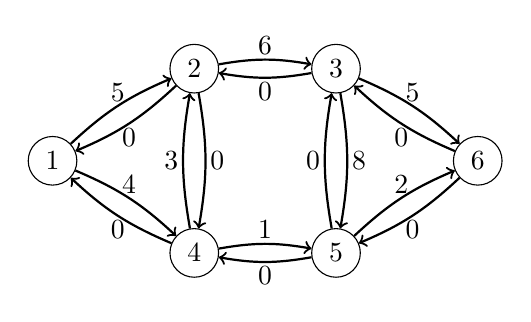
\begin{tikzpicture}[scale=0.9,label distance=-2mm]
		\node[draw, circle] (1) at (1,1.3) {$1$};
		\node[draw, circle] (2) at (3,2.6) {$2$};
		\node[draw, circle] (3) at (5,2.6) {$3$};
		\node[draw, circle] (4) at (7,1.3) {$6$};
		\node[draw, circle] (5) at (3,0) {$4$};
		\node[draw, circle] (6) at (5,0) {$5$};

		\path[draw,thick,->] (1) edge [bend left=10] node[font=\small,label=5] {} (2);
		\path[draw,thick,->] (2) edge [bend left=10] node[font=\small,label=below:0] {} (1);
		\path[draw,thick,->] (2) edge [bend left=10] node[font=\small,label=6] {} (3);
		\path[draw,thick,->] (3) edge [bend left=10] node[font=\small,label=below:0] {} (2);
		\path[draw,thick,->] (3) edge [bend left=10] node[font=\small,label=5] {} (4);
		\path[draw,thick,->] (4) edge [bend left=10] node[font=\small,label=below:0] {} (3);
		\path[draw,thick,->] (1) edge [bend left=10] node[font=\small,label=4] {} (5);
		\path[draw,thick,->] (5) edge [bend left=10] node[font=\small,label=below:0] {} (1);
		\path[draw,thick,->] (5) edge [bend left=10] node[font=\small,label=1] {} (6);
		\path[draw,thick,->] (6) edge [bend left=10] node[font=\small,label=below:0] {} (5);
		\path[draw,thick,->] (6) edge [bend left=10] node[font=\small,label=2] {} (4);
		\path[draw,thick,->] (4) edge [bend left=10] node[font=\small,label=below:0] {} (6);
		\path[draw,thick,->] (5) edge [bend left=10] node[font=\small,label=left:3] {} (2);
		\path[draw,thick,->] (2) edge [bend left=10] node[font=\small,label=right:0] {} (5);
		\path[draw,thick,->] (3) edge [bend left=10] node[font=\small,label=right:8] {} (6);
		\path[draw,thick,->] (6) edge [bend left=10] node[font=\small,label=left:0] {} (3);
		\end{tikzpicture}
	\end{center}
\end{samepage}

\subsubsection{Descripci\'on del algoritmo}

El algoritmo de Ford–Fulkerson consta de varias
iteraciones.
En cada iteraci\'on, el algoritmo encuentra
un camino desde la fuente hacia el sumidero
de tal forma que cada arista en el camino tenga un peso positivo.
Si existe m\'as de un camino posible,
se puede seleccionar cualquiera de ellos.

Por ejemplo, supongamos que seleccionamos el siguiente camino:

\begin{center}
	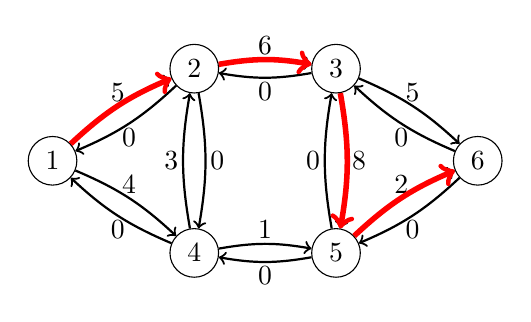
\begin{tikzpicture}[scale=0.9,label distance=-2mm]
	\node[draw, circle] (1) at (1,1.3) {$1$};
	\node[draw, circle] (2) at (3,2.6) {$2$};
	\node[draw, circle] (3) at (5,2.6) {$3$};
	\node[draw, circle] (4) at (7,1.3) {$6$};
	\node[draw, circle] (5) at (3,0) {$4$};
	\node[draw, circle] (6) at (5,0) {$5$};

	\path[draw,thick,->] (1) edge [bend left=10] node[font=\small,label=5] {} (2);
	\path[draw,thick,->] (2) edge [bend left=10] node[font=\small,label=below:0] {} (1);
	\path[draw,thick,->] (2) edge [bend left=10] node[font=\small,label=6] {} (3);
	\path[draw,thick,->] (3) edge [bend left=10] node[font=\small,label=below:0] {} (2);
	\path[draw,thick,->] (3) edge [bend left=10] node[font=\small,label=5] {} (4);
	\path[draw,thick,->] (4) edge [bend left=10] node[font=\small,label=below:0] {} (3);
	\path[draw,thick,->] (1) edge [bend left=10] node[font=\small,label=4] {} (5);
	\path[draw,thick,->] (5) edge [bend left=10] node[font=\small,label=below:0] {} (1);
	\path[draw,thick,->] (5) edge [bend left=10] node[font=\small,label=1] {} (6);
	\path[draw,thick,->] (6) edge [bend left=10] node[font=\small,label=below:0] {} (5);
	\path[draw,thick,->] (6) edge [bend left=10] node[font=\small,label=2] {} (4);
	\path[draw,thick,->] (4) edge [bend left=10] node[font=\small,label=below:0] {} (6);
	\path[draw,thick,->] (5) edge [bend left=10] node[font=\small,label=left:3] {} (2);
	\path[draw,thick,->] (2) edge [bend left=10] node[font=\small,label=right:0] {} (5);
	\path[draw,thick,->] (3) edge [bend left=10] node[font=\small,label=right:8] {} (6);
	\path[draw,thick,->] (6) edge [bend left=10] node[font=\small,label=left:0] {} (3);

	\path[draw=red,thick,->,line width=2pt] (1) edge [bend left=10] (2);
	\path[draw=red,thick,->,line width=2pt] (2) edge [bend left=10] (3);
	\path[draw=red,thick,->,line width=2pt] (3) edge [bend left=10] (6);
	\path[draw=red,thick,->,line width=2pt] (6) edge [bend left=10] (4);
	\end{tikzpicture}
\end{center}

Despu\'es de seleccionar el camino, el flujo incrementa en $x$ unidades,
donde $x$ es el menor peso de las aristas que componen el camino.
Adem\'as, el peso de cada arista en el camino
es decrementado en $x$ unidades y el peso de cada arista reversa
es incrementado en $x$ unidades.

En el camino anterior, los pesos de
las aristas son 5, 6, 8 y 2.
El menor peso es 2,
de esa manera el flujo incrementa en 2 unidades
y el nuevo grafo queda de la siguiente forma:

\begin{center}
	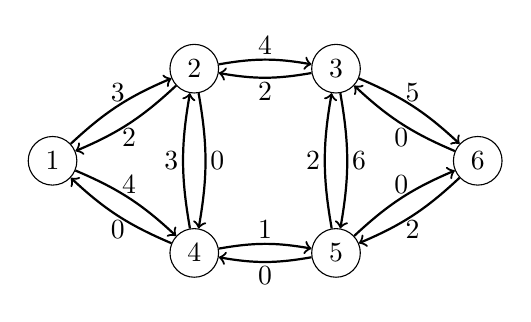
\begin{tikzpicture}[scale=0.9,label distance=-2mm]
	\node[draw, circle] (1) at (1,1.3) {$1$};
	\node[draw, circle] (2) at (3,2.6) {$2$};
	\node[draw, circle] (3) at (5,2.6) {$3$};
	\node[draw, circle] (4) at (7,1.3) {$6$};
	\node[draw, circle] (5) at (3,0) {$4$};
	\node[draw, circle] (6) at (5,0) {$5$};

	\path[draw,thick,->] (1) edge [bend left=10] node[font=\small,label=3] {} (2);
	\path[draw,thick,->] (2) edge [bend left=10] node[font=\small,label=below:2] {} (1);
	\path[draw,thick,->] (2) edge [bend left=10] node[font=\small,label=4] {} (3);
	\path[draw,thick,->] (3) edge [bend left=10] node[font=\small,label=below:2] {} (2);
	\path[draw,thick,->] (3) edge [bend left=10] node[font=\small,label=5] {} (4);
	\path[draw,thick,->] (4) edge [bend left=10] node[font=\small,label=below:0] {} (3);
	\path[draw,thick,->] (1) edge [bend left=10] node[font=\small,label=4] {} (5);
	\path[draw,thick,->] (5) edge [bend left=10] node[font=\small,label=below:0] {} (1);
	\path[draw,thick,->] (5) edge [bend left=10] node[font=\small,label=1] {} (6);
	\path[draw,thick,->] (6) edge [bend left=10] node[font=\small,label=below:0] {} (5);
	\path[draw,thick,->] (6) edge [bend left=10] node[font=\small,label=0] {} (4);
	\path[draw,thick,->] (4) edge [bend left=10] node[font=\small,label=below:2] {} (6);
	\path[draw,thick,->] (5) edge [bend left=10] node[font=\small,label=left:3] {} (2);
	\path[draw,thick,->] (2) edge [bend left=10] node[font=\small,label=right:0] {} (5);
	\path[draw,thick,->] (3) edge [bend left=10] node[font=\small,label=right:6] {} (6);
	\path[draw,thick,->] (6) edge [bend left=10] node[font=\small,label=left:2] {} (3);
	\end{tikzpicture}
\end{center}

Se puede asegurar que el incremento del flujo implica un decrecimiento
en la cantidad de flujo que puede pasar por las aristas en el futuro.
Por otra parte, es posible modificar despu\'es el
flujo utilizando las aristas reversas del grafo
en caso de que sea
beneficioso dirigir el flujo por otro camino.

El algoritmo incrementa el flujo siempre que
exista un camino desde la fuente hacia
el sumidero pasando por aristas con pesos positivos.
En el ejemplo actual, nuestro camino siguiente puede ser como se muestra a continuaci\'on:

\begin{center}
	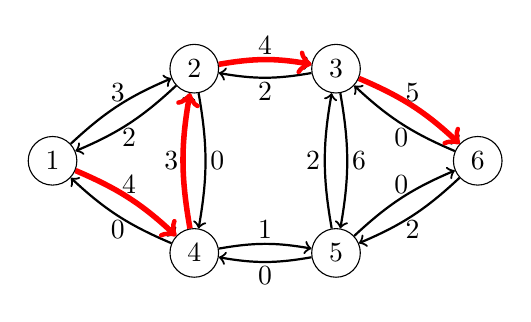
\begin{tikzpicture}[scale=0.9,label distance=-2mm]
	\node[draw, circle] (1) at (1,1.3) {$1$};
	\node[draw, circle] (2) at (3,2.6) {$2$};
	\node[draw, circle] (3) at (5,2.6) {$3$};
	\node[draw, circle] (4) at (7,1.3) {$6$};
	\node[draw, circle] (5) at (3,0) {$4$};
	\node[draw, circle] (6) at (5,0) {$5$};

	\path[draw,thick,->] (1) edge [bend left=10] node[font=\small,label=3] {} (2);
	\path[draw,thick,->] (2) edge [bend left=10] node[font=\small,label=below:2] {} (1);
	\path[draw,thick,->] (2) edge [bend left=10] node[font=\small,label=4] {} (3);
	\path[draw,thick,->] (3) edge [bend left=10] node[font=\small,label=below:2] {} (2);
	\path[draw,thick,->] (3) edge [bend left=10] node[font=\small,label=5] {} (4);
	\path[draw,thick,->] (4) edge [bend left=10] node[font=\small,label=below:0] {} (3);
	\path[draw,thick,->] (1) edge [bend left=10] node[font=\small,label=4] {} (5);
	\path[draw,thick,->] (5) edge [bend left=10] node[font=\small,label=below:0] {} (1);
	\path[draw,thick,->] (5) edge [bend left=10] node[font=\small,label=1] {} (6);
	\path[draw,thick,->] (6) edge [bend left=10] node[font=\small,label=below:0] {} (5);
	\path[draw,thick,->] (6) edge [bend left=10] node[font=\small,label=0] {} (4);
	\path[draw,thick,->] (4) edge [bend left=10] node[font=\small,label=below:2] {} (6);
	\path[draw,thick,->] (5) edge [bend left=10] node[font=\small,label=left:3] {} (2);
	\path[draw,thick,->] (2) edge [bend left=10] node[font=\small,label=right:0] {} (5);
	\path[draw,thick,->] (3) edge [bend left=10] node[font=\small,label=right:6] {} (6);
	\path[draw,thick,->] (6) edge [bend left=10] node[font=\small,label=left:2] {} (3);

	\path[draw=red,thick,->,line width=2pt] (1) edge [bend left=10] (5);
	\path[draw=red,thick,->,line width=2pt] (5) edge [bend left=10] (2);
	\path[draw=red,thick,->,line width=2pt] (2) edge [bend left=10] (3);
	\path[draw=red,thick,->,line width=2pt] (3) edge [bend left=10] (4);
	\end{tikzpicture}
\end{center}

El menor peso en este camino es 3,
incrementando de esta forma el flujo en 3 a lo largo del camino,
y el flujo total luego de procesar el camino es 5.

\begin{samepage}
	El nuevo grafo queda de la siguiente forma:

	\begin{center}
		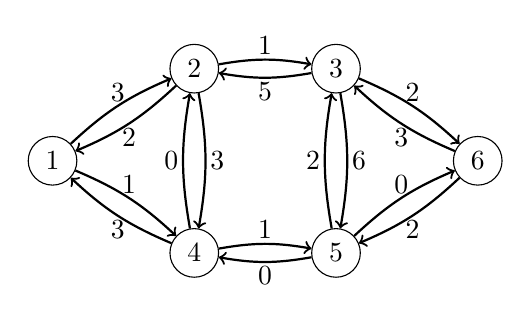
\begin{tikzpicture}[scale=0.9,label distance=-2mm]
		\node[draw, circle] (1) at (1,1.3) {$1$};
		\node[draw, circle] (2) at (3,2.6) {$2$};
		\node[draw, circle] (3) at (5,2.6) {$3$};
		\node[draw, circle] (4) at (7,1.3) {$6$};
		\node[draw, circle] (5) at (3,0) {$4$};
		\node[draw, circle] (6) at (5,0) {$5$};

		\path[draw,thick,->] (1) edge [bend left=10] node[font=\small,label=3] {} (2);
		\path[draw,thick,->] (2) edge [bend left=10] node[font=\small,label=below:2] {} (1);
		\path[draw,thick,->] (2) edge [bend left=10] node[font=\small,label=1] {} (3);
		\path[draw,thick,->] (3) edge [bend left=10] node[font=\small,label=below:5] {} (2);
		\path[draw,thick,->] (3) edge [bend left=10] node[font=\small,label=2] {} (4);
		\path[draw,thick,->] (4) edge [bend left=10] node[font=\small,label=below:3] {} (3);
		\path[draw,thick,->] (1) edge [bend left=10] node[font=\small,label=1] {} (5);
		\path[draw,thick,->] (5) edge [bend left=10] node[font=\small,label=below:3] {} (1);
		\path[draw,thick,->] (5) edge [bend left=10] node[font=\small,label=1] {} (6);
		\path[draw,thick,->] (6) edge [bend left=10] node[font=\small,label=below:0] {} (5);
		\path[draw,thick,->] (6) edge [bend left=10] node[font=\small,label=0] {} (4);
		\path[draw,thick,->] (4) edge [bend left=10] node[font=\small,label=below:2] {} (6);
		\path[draw,thick,->] (5) edge [bend left=10] node[font=\small,label=left:0] {} (2);
		\path[draw,thick,->] (2) edge [bend left=10] node[font=\small,label=right:3] {} (5);
		\path[draw,thick,->] (3) edge [bend left=10] node[font=\small,label=right:6] {} (6);
		\path[draw,thick,->] (6) edge [bend left=10] node[font=\small,label=left:2] {} (3);
		\end{tikzpicture}
	\end{center}
\end{samepage}

A\'un se necesitan dos iteraciones m\'as para alcanzar el flujo m\'aximo.
Por ejemplo, podemos escoger los caminos
$1 \rightarrow 2 \rightarrow 3 \rightarrow 6$ y
$1 \rightarrow 4 \rightarrow 5 \rightarrow 3 \rightarrow 6$.
Ambos caminos incrementan el flujo en 1,
quedando el grafo final como se muestra a continuaci\'on:

\begin{center}
	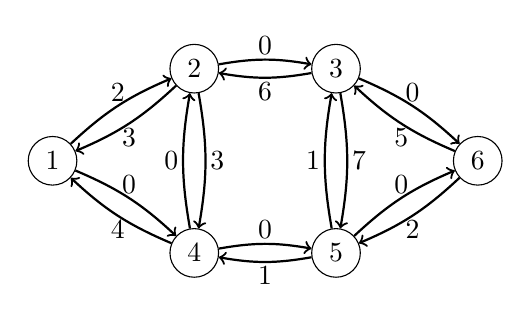
\begin{tikzpicture}[scale=0.9,label distance=-2mm]
	\node[draw, circle] (1) at (1,1.3) {$1$};
	\node[draw, circle] (2) at (3,2.6) {$2$};
	\node[draw, circle] (3) at (5,2.6) {$3$};
	\node[draw, circle] (4) at (7,1.3) {$6$};
	\node[draw, circle] (5) at (3,0) {$4$};
	\node[draw, circle] (6) at (5,0) {$5$};

	\path[draw,thick,->] (1) edge [bend left=10] node[font=\small,label=2] {} (2);
	\path[draw,thick,->] (2) edge [bend left=10] node[font=\small,label=below:3] {} (1);
	\path[draw,thick,->] (2) edge [bend left=10] node[font=\small,label=0] {} (3);
	\path[draw,thick,->] (3) edge [bend left=10] node[font=\small,label=below:6] {} (2);
	\path[draw,thick,->] (3) edge [bend left=10] node[font=\small,label=0] {} (4);
	\path[draw,thick,->] (4) edge [bend left=10] node[font=\small,label=below:5] {} (3);
	\path[draw,thick,->] (1) edge [bend left=10] node[font=\small,label=0] {} (5);
	\path[draw,thick,->] (5) edge [bend left=10] node[font=\small,label=below:4] {} (1);
	\path[draw,thick,->] (5) edge [bend left=10] node[font=\small,label=0] {} (6);
	\path[draw,thick,->] (6) edge [bend left=10] node[font=\small,label=below:1] {} (5);
	\path[draw,thick,->] (6) edge [bend left=10] node[font=\small,label=0] {} (4);
	\path[draw,thick,->] (4) edge [bend left=10] node[font=\small,label=below:2] {} (6);
	\path[draw,thick,->] (5) edge [bend left=10] node[font=\small,label=left:0] {} (2);
	\path[draw,thick,->] (2) edge [bend left=10] node[font=\small,label=right:3] {} (5);
	\path[draw,thick,->] (3) edge [bend left=10] node[font=\small,label=right:7] {} (6);
	\path[draw,thick,->] (6) edge [bend left=10] node[font=\small,label=left:1] {} (3);
	\end{tikzpicture}
\end{center}

Ya no es posible incrementar m\'as el flujo,
debido a que no existe un camino desde la fuente
hacia el sumidero formado por aristas con peso positivo.
Por lo tanto, el algoritmo termina y el flujo m\'aximo es 7.

\subsubsection{Encontrando caminos}

El algoritmo de Ford–Fulkerson no especifica
como debemos seleccionar los caminos que incrementan el flujo.
De cualquier forma, el algoritmo termina en alg\'un momento
y encuentra de manera correcta el flujo m\'aximo.
Sin embargo, la eficiencia del algoritmo depende en
la forma en que los caminos son seleccionados.

Una forma sencilla de encontrar caminos es mediante la b\'usqueda en profundidad.
En la mayor\'ia de los casos, esta funciona bien, pero en el peor caso,
cada camino incrementa el flujo solamente en una unidad
y el algoritmo se torna lento.
Afortunadamente, esta situaci\'on se puede evitar
utilizando una de las t\'ecnicas que se detallan a continuaci\'on:

\index{algoritmo de Edmonds–Karp}

El algoritmo de \key{Edmonds–Karp} \cite{edm72}
selecciona en cada iteraci\'on el camino
con la menor cantidad de aristas posible.
Esto se puede lograr mediante la b\'usqueda a lo ancho
en vez de la b\'usqueda en profundidad para encontrar los caminos.
De esta forma se garantiza el incremento
r\'apido del flujo, la complejidad temporal de
este algoritmo es $O(m^2 n)$.

\index{algoritmo de escalado}

El \key{algoritmo de escalado} \cite{ahu91} usa b\'usqueda en profundidad
para encontrar caminos donde el peso de las aristas
sea mayor o igual que un umbral.
Al inicio, el umbral tiene como valor
la suma de las capacidades de las aristas
que comienzan en la fuente.
Cada vez que no se puede encontrar un camino,
se divide el umbral entre 2.
La complejidad temporal de este algoritmo es $O(m^2 \log c)$,
donde $c$ es el valor inicial del umbral.

En la pr\'actica, el algoritmo de escalado es m\'as f\'acil de implementar,
debido a que se encuentran los caminos mediante la b\'usqueda en profundidad.
Ambos algoritmos son lo suficientemente eficientes
para resolver los problemas que usualmente aparecen en las competencias.

\subsubsection{Cortes m\'inimos}

\index{corte m\'inimo}

Resulta que una vez que el algoritmo de Ford–Fulkerson
ha encontrado un flujo m\'aximo,
tambi\'en ha encontrado un corte m\'inimo.
Sea $A$ el conjunto de nodos
que pueden ser alcanzados desde la fuente
utilizando aristas con pesos positivos.
En el grafo de ejemplo, $A$ contiene los nodos 1, 2 y 4:

\begin{center}
	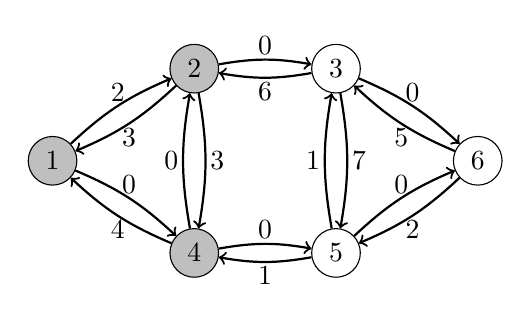
\begin{tikzpicture}[scale=0.9,label distance=-2mm]
	\node[draw, circle,fill=lightgray] (1) at (1,1.3) {$1$};
	\node[draw, circle,fill=lightgray] (2) at (3,2.6) {$2$};
	\node[draw, circle] (3) at (5,2.6) {$3$};
	\node[draw, circle] (4) at (7,1.3) {$6$};
	\node[draw, circle,fill=lightgray] (5) at (3,0) {$4$};
	\node[draw, circle] (6) at (5,0) {$5$};

	\path[draw,thick,->] (1) edge [bend left=10] node[font=\small,label=2] {} (2);
	\path[draw,thick,->] (2) edge [bend left=10] node[font=\small,label=below:3] {} (1);
	\path[draw,thick,->] (2) edge [bend left=10] node[font=\small,label=0] {} (3);
	\path[draw,thick,->] (3) edge [bend left=10] node[font=\small,label=below:6] {} (2);
	\path[draw,thick,->] (3) edge [bend left=10] node[font=\small,label=0] {} (4);
	\path[draw,thick,->] (4) edge [bend left=10] node[font=\small,label=below:5] {} (3);
	\path[draw,thick,->] (1) edge [bend left=10] node[font=\small,label=0] {} (5);
	\path[draw,thick,->] (5) edge [bend left=10] node[font=\small,label=below:4] {} (1);
	\path[draw,thick,->] (5) edge [bend left=10] node[font=\small,label=0] {} (6);
	\path[draw,thick,->] (6) edge [bend left=10] node[font=\small,label=below:1] {} (5);
	\path[draw,thick,->] (6) edge [bend left=10] node[font=\small,label=0] {} (4);
	\path[draw,thick,->] (4) edge [bend left=10] node[font=\small,label=below:2] {} (6);
	\path[draw,thick,->] (5) edge [bend left=10] node[font=\small,label=left:0] {} (2);
	\path[draw,thick,->] (2) edge [bend left=10] node[font=\small,label=right:3] {} (5);
	\path[draw,thick,->] (3) edge [bend left=10] node[font=\small,label=right:7] {} (6);
	\path[draw,thick,->] (6) edge [bend left=10] node[font=\small,label=left:1] {} (3);
	\end{tikzpicture}
\end{center}

Ahora el corte m\'inimo est\'a formado por las aristas del grafo original
que comienzan en alg\'un nodo de $A$, terminan en alg\'un nodo que no pertenece a $A$,
y cuyas capacidades est\'an saturadas
por el flujo m\'aximo.
En el grafo anterior, esas aristas son
$2 \rightarrow 3$ y $4 \rightarrow 5$,
que corresponden al corte m\'inimo $6+1=7$.

Por qu\'e el flujo producido por el algoritmo es m\'aximo
y por qu\'e el corte es m\'inimo?
Esto se debe a que el grafo no puede
contener un flujo de tama\~no mayor
que el peso de cualquier corte en el grafo.
Por lo tanto, siempre que el flujo y el corte sean iguales en tama\~no,
se puede asegurar que el flujo es m\'aximo y el corte es m\'inimo

Tomemos en consideraci\'on cualquier corte en el grafo
tal que la fuente pertenezca a $A$,
el sumidero pertenezca a $B$
y existan aristas entre ambos conjuntos:

\begin{center}
	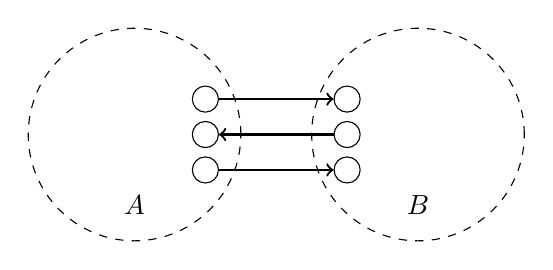
\begin{tikzpicture}[scale=0.9]
	\draw[dashed] (-2,0) circle (1.5);
	\draw[dashed] (2,0) circle (1.5);

	\node at (-2,-1) {$A$};
	\node at (2,-1) {$B$};

	\node[draw, circle] (1) at (-1,0.5) {};
	\node[draw, circle] (2) at (-1,0) {};
	\node[draw, circle] (3) at (-1,-0.5) {};
	\node[draw, circle] (4) at (1,0.5) {};
	\node[draw, circle] (5) at (1,0) {};
	\node[draw, circle] (6) at (1,-0.5) {};

	\path[draw,thick,->] (1) -- (4);
	\path[draw,thick,->] (5) -- (2);
	\path[draw,thick,->] (3) -- (6);

	\end{tikzpicture}
\end{center}

El tama\~no del corte es la suma de las aristas
que van desde el conjunto $A$ hacia el conjunto $B$.
Esto es una cuota m\'axima para el flujo
en el grafo, porque el flujo tiene que proceder
desde el conjunto $A$ hacia el conjunto $B$.
Por lo tanto, un flujo m\'aximo es menor o igual
que cualquier corte del grafo.

Por otra parte, el algoritmo de Ford–Fulkerson
produce un flujo que es \emph{exactamente} tan grande
como lo es un corte en el grafo.
As\'i, el flujo tiene que ser un flujo m\'aximo
y el corte tiene que ser un corte m\'inimo.

\section{Caminos disjuntos}

Muchos problemas de grafos se pueden resolver
mediante una reducci\'on al problema del flujo m\'aximo.
Nuestro primer ejmplo de un problema de este tipo
lo detallamos a continuaci\'on: tenemos un grafo dirigido
con una fuente y un sumidero,
y tenemos que encontrar la m\'axima cantidad
de caminos disjuntos desde la fuente hacia el sumidero.

\subsubsection{Caminos disjuntos en las aristas}

Primero nos concentraremos en el problema
de encontrar la mayor cantidad de
\key{caminos disjuntos en las aristas} desde la fuente hacia el sumidero.
Esto significa que debemos encontrar un conjunto de caminos
donde cada arista aparezca a lo sumo en un solo camino.

Por ejemplo, considera el grafo siguiente:
\begin{center}
	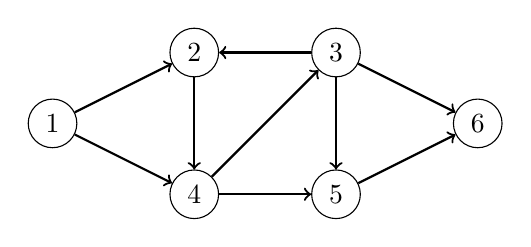
\begin{tikzpicture}[scale=0.9]
	\node[draw, circle] (1) at (1,2) {$1$};
	\node[draw, circle] (2) at (3,3) {$2$};
	\node[draw, circle] (3) at (5,3) {$3$};
	\node[draw, circle] (4) at (3,1) {$4$};
	\node[draw, circle] (5) at (5,1) {$5$};
	\node[draw, circle] (6) at (7,2) {$6$};
	\path[draw,thick,->] (1) -- (2);
	\path[draw,thick,->] (1) -- (4);
	\path[draw,thick,->] (2) -- (4);
	\path[draw,thick,->] (3) -- (2);
	\path[draw,thick,->] (3) -- (5);
	\path[draw,thick,->] (3) -- (6);
	\path[draw,thick,->] (4) -- (3);
	\path[draw,thick,->] (4) -- (5);
	\path[draw,thick,->] (5) -- (6);
	\end{tikzpicture}
\end{center}

En este grafo, la cantidad m\'axima de caminos
disjuntos en las aristas es 2.
Se pueden seleccionar los caminos
$1 \rightarrow 2 \rightarrow 4 \rightarrow 3 \rightarrow 6$
y $1 \rightarrow 4 \rightarrow 5 \rightarrow 6$ de la siguiente forma:

\begin{center}
	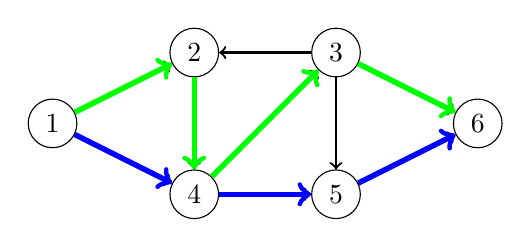
\begin{tikzpicture}[scale=0.9]
	\node[draw, circle] (1) at (1,2) {$1$};
	\node[draw, circle] (2) at (3,3) {$2$};
	\node[draw, circle] (3) at (5,3) {$3$};
	\node[draw, circle] (4) at (3,1) {$4$};
	\node[draw, circle] (5) at (5,1) {$5$};
	\node[draw, circle] (6) at (7,2) {$6$};
	\path[draw,thick,->] (1) -- (2);
	\path[draw,thick,->] (1) -- (4);
	\path[draw,thick,->] (2) -- (4);
	\path[draw,thick,->] (3) -- (2);
	\path[draw,thick,->] (3) -- (5);
	\path[draw,thick,->] (3) -- (6);
	\path[draw,thick,->] (4) -- (3);
	\path[draw,thick,->] (4) -- (5);
	\path[draw,thick,->] (5) -- (6);

	\path[draw=green,thick,->,line width=2pt] (1) -- (2);
	\path[draw=green,thick,->,line width=2pt] (2) -- (4);
	\path[draw=green,thick,->,line width=2pt] (4) -- (3);
	\path[draw=green,thick,->,line width=2pt] (3) -- (6);

	\path[draw=blue,thick,->,line width=2pt] (1) -- (4);
	\path[draw=blue,thick,->,line width=2pt] (4) -- (5);
	\path[draw=blue,thick,->,line width=2pt] (5) -- (6);
	\end{tikzpicture}
\end{center}

Resulta que la cantidad m\'axima de
caminos disjuntos en las aristas
es igual al flujo m\'aximo en el grafo,
asumiendo que la capacidad de cada arista es 1.
Luego de construirse el flujo m\'aximo,
los caminos disjuntos en las aristas se pueden encontrar
de manera \'avida al seguir los caminos desde la fuente hacia el sumidero.

\subsubsection{Caminos disjuntos en los nodos}

Tomemos en consideraci\'on otro problema:
encontrar la cantidad m\'axima de
\key{caminos disjuntos en los nodos} desde la fuente
hacia el sumidero.
En este problema, cada nodo,
con excepci\'on de la fuente y el sumidero,
pueden aparecer a lo sumo en un camino.
La cantidad de caminos disjuntos en los nodos es
usualmente menor que la cantidad de
caminos disjuntos en las aristas.

Por ejemplo, en el grafo anterior,
la mayor cantidad de caminos disjuntos en los nodos es 1:

\begin{center}
	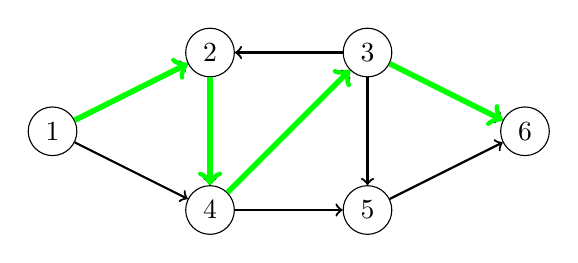
\begin{tikzpicture}
	\node[draw, circle] (1) at (1,2) {$1$};
	\node[draw, circle] (2) at (3,3) {$2$};
	\node[draw, circle] (3) at (5,3) {$3$};
	\node[draw, circle] (4) at (3,1) {$4$};
	\node[draw, circle] (5) at (5,1) {$5$};
	\node[draw, circle] (6) at (7,2) {$6$};
	\path[draw,thick,->] (1) -- (2);
	\path[draw,thick,->] (1) -- (4);
	\path[draw,thick,->] (2) -- (4);
	\path[draw,thick,->] (3) -- (2);
	\path[draw,thick,->] (3) -- (5);
	\path[draw,thick,->] (3) -- (6);
	\path[draw,thick,->] (4) -- (3);
	\path[draw,thick,->] (4) -- (5);
	\path[draw,thick,->] (5) -- (6);

	\path[draw=green,thick,->,line width=2pt] (1) -- (2);
	\path[draw=green,thick,->,line width=2pt] (2) -- (4);
	\path[draw=green,thick,->,line width=2pt] (4) -- (3);
	\path[draw=green,thick,->,line width=2pt] (3) -- (6);
	\end{tikzpicture}
\end{center}

Tambi\'en podemos reducir este problema al problema de flujo m\'aximo.
Dado que cada nodo puede aparecer a lo sumo en un camino,
tenemos que limitar el flujo que pasa por los nodos.
Una forma est\'andar de lograr esto es dividiendo cada nodo en dos nodos
tal que el primer nodo tiene las aristas entrantes
del nodo original y el segundo nodo tiene las aristas salientes
del nodo original.
Adem\'as, se crea nueva arista desde el primer nodo
hacia el segundo nodo.

En nuestro ejemplo, el grafo queda de la siguiente forma:
\begin{center}
	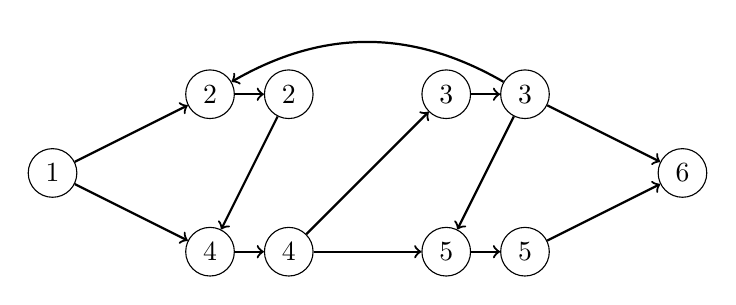
\begin{tikzpicture}
	\node[draw, circle] (1) at (1,2) {$1$};

	\node[draw, circle] (2a) at (3,3) {$2$};
	\node[draw, circle] (3a) at (6,3) {$3$};
	\node[draw, circle] (4a) at (3,1) {$4$};
	\node[draw, circle] (5a) at (6,1) {$5$};

	\node[draw, circle] (2b) at (4,3) {$2$};
	\node[draw, circle] (3b) at (7,3) {$3$};
	\node[draw, circle] (4b) at (4,1) {$4$};
	\node[draw, circle] (5b) at (7,1) {$5$};

	\node[draw, circle] (6) at (9,2) {$6$};

	\path[draw,thick,->] (2a) -- (2b);
	\path[draw,thick,->] (3a) -- (3b);
	\path[draw,thick,->] (4a) -- (4b);
	\path[draw,thick,->] (5a) -- (5b);

	\path[draw,thick,->] (1) -- (2a);
	\path[draw,thick,->] (1) -- (4a);
	\path[draw,thick,->] (2b) -- (4a);
	\path[draw,thick,->] (3b) edge [bend right=30] (2a);
	\path[draw,thick,->] (3b) -- (5a);
	\path[draw,thick,->] (3b) -- (6);
	\path[draw,thick,->] (4b) -- (3a);
	\path[draw,thick,->] (4b) -- (5a);
	\path[draw,thick,->] (5b) -- (6);
	\end{tikzpicture}
\end{center}

El flujo m\'aximo en el grafo queda como se muestra a continuaci\'on:
\begin{center}
	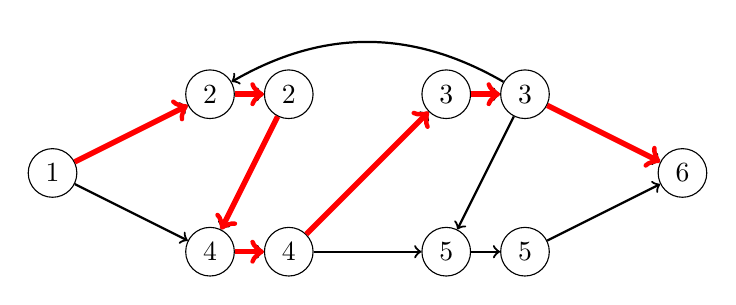
\begin{tikzpicture}
	\node[draw, circle] (1) at (1,2) {$1$};

	\node[draw, circle] (2a) at (3,3) {$2$};
	\node[draw, circle] (3a) at (6,3) {$3$};
	\node[draw, circle] (4a) at (3,1) {$4$};
	\node[draw, circle] (5a) at (6,1) {$5$};

	\node[draw, circle] (2b) at (4,3) {$2$};
	\node[draw, circle] (3b) at (7,3) {$3$};
	\node[draw, circle] (4b) at (4,1) {$4$};
	\node[draw, circle] (5b) at (7,1) {$5$};

	\node[draw, circle] (6) at (9,2) {$6$};

	\path[draw,thick,->] (2a) -- (2b);
	\path[draw,thick,->] (3a) -- (3b);
	\path[draw,thick,->] (4a) -- (4b);
	\path[draw,thick,->] (5a) -- (5b);

	\path[draw,thick,->] (1) -- (2a);
	\path[draw,thick,->] (1) -- (4a);
	\path[draw,thick,->] (2b) -- (4a);
	\path[draw,thick,->] (3b) edge [bend right=30] (2a);
	\path[draw,thick,->] (3b) -- (5a);
	\path[draw,thick,->] (3b) -- (6);
	\path[draw,thick,->] (4b) -- (3a);
	\path[draw,thick,->] (4b) -- (5a);
	\path[draw,thick,->] (5b) -- (6);

	\path[draw=red,thick,->,line width=2pt] (1) -- (2a);
	\path[draw=red,thick,->,line width=2pt] (2a) -- (2b);
	\path[draw=red,thick,->,line width=2pt] (2b) -- (4a);
	\path[draw=red,thick,->,line width=2pt] (4a) -- (4b);
	\path[draw=red,thick,->,line width=2pt] (4b) -- (3a);
	\path[draw=red,thick,->,line width=2pt] (3a) -- (3b);
	\path[draw=red,thick,->,line width=2pt] (3b) -- (6);
	\end{tikzpicture}
\end{center}

Por lo tanto, la cantidad m\'axima de caminos disjuntos en los nodos
desde la fuente hacia el sumidero es 1.

\section{Emparejamiento m\'aximo}

\index{emparejamiento}
\index{emparejamiento m\'aximo}

El problema del \key{emparejamiento m\'aximo} consiste en encontrar
un conjunto m\'aximo de pares de nodos en un grafo
donde cada par est\'e conectado por una arista
y cada nodo pertenezca a lo sumo a un par.

Existen algoritmos polinomiales para encontrar
emparejamientos m\'aximos en grafos generales \cite{edm65},
pero tales algoritmos son bastante complejos y no
aparecen en los concursos de programaci\'on.
Sin embargo, en grafos bipartitos,
el problema del emparejamiento m\'aximo es mucho m\'as sencillo
de resolver, debido a que podemos reducirlo al
problema del flujo m\'aximo.

\subsubsection{Encontrando emparejamientos m\'aximos}

Los nodos de un grafo bipartito se pueden dividir
siempre en dos grupos donde todas las aristas
del grafo van desde el grupo izquierdo hacia el grupo derecho.
Por ejemplo, considera el siguiente grafo bipartito:

\begin{center}
	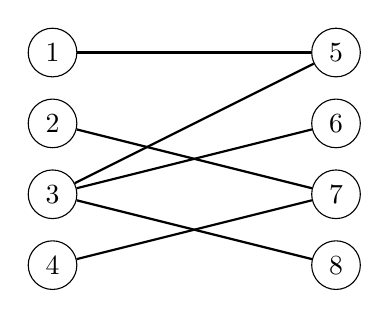
\begin{tikzpicture}[scale=0.60]
	\node[draw, circle] (1) at (2,4.5) {1};
	\node[draw, circle] (2) at (2,3) {2};
	\node[draw, circle] (3) at (2,1.5) {3};
	\node[draw, circle] (4) at (2,0) {4};
	\node[draw, circle] (5) at (8,4.5) {5};
	\node[draw, circle] (6) at (8,3) {6};
	\node[draw, circle] (7) at (8,1.5) {7};
	\node[draw, circle] (8) at (8,0) {8};

	\path[draw,thick,-] (1) -- (5);
	\path[draw,thick,-] (2) -- (7);
	\path[draw,thick,-] (3) -- (5);
	\path[draw,thick,-] (3) -- (6);
	\path[draw,thick,-] (3) -- (8);
	\path[draw,thick,-] (4) -- (7);
	\end{tikzpicture}
\end{center}

En este grafo, el tama\~no del emparejamiento m\'aximo es 3:
\begin{center}
	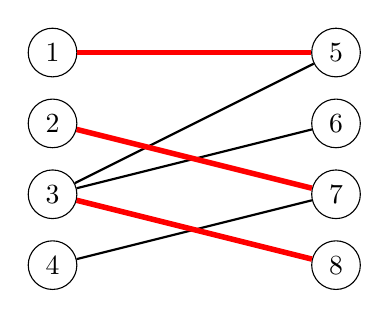
\begin{tikzpicture}[scale=0.60]
	\node[draw, circle] (1) at (2,4.5) {1};
	\node[draw, circle] (2) at (2,3) {2};
	\node[draw, circle] (3) at (2,1.5) {3};
	\node[draw, circle] (4) at (2,0) {4};
	\node[draw, circle] (5) at (8,4.5) {5};
	\node[draw, circle] (6) at (8,3) {6};
	\node[draw, circle] (7) at (8,1.5) {7};
	\node[draw, circle] (8) at (8,0) {8};

	\path[draw,thick,-] (1) -- (5);
	\path[draw,thick,-] (2) -- (7);
	\path[draw,thick,-] (3) -- (5);
	\path[draw,thick,-] (3) -- (6);
	\path[draw,thick,-] (3) -- (8);
	\path[draw,thick,-] (4) -- (7);

	\path[draw=red,thick,-,line width=2pt] (1) -- (5);
	\path[draw=red,thick,-,line width=2pt] (2) -- (7);
	\path[draw=red,thick,-,line width=2pt] (3) -- (8);
	\end{tikzpicture}
\end{center}

Podemos reducir el problema del emparejamiento m\'aximo
al problema del flujo m\'aximo a\~nadiendo dos nodos nuevos
al grafo: una fuente y un sumidero.
Adem\'as, agregamos aristas desde la fuente
hacia cada nodo de la izquierda y desde cada nodo de la derecha hacia el sumidero.
Como resultado, se obtiene que el flujo m\'aximo del grafo
es igual al emparejamiento m\'aximo del grafo original.

Como ejemplo se muestra a continuaci\'on la
reducci\'on para el grafo anterior:
\begin{center}
	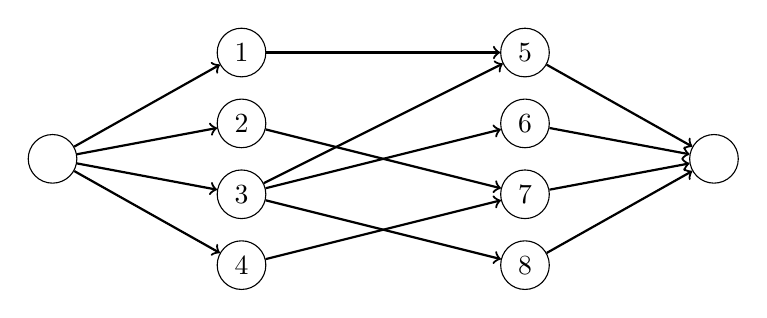
\begin{tikzpicture}[scale=0.60]
	\node[draw, circle] (1) at (2,4.5) {1};
	\node[draw, circle] (2) at (2,3) {2};
	\node[draw, circle] (3) at (2,1.5) {3};
	\node[draw, circle] (4) at (2,0) {4};
	\node[draw, circle] (5) at (8,4.5) {5};
	\node[draw, circle] (6) at (8,3) {6};
	\node[draw, circle] (7) at (8,1.5) {7};
	\node[draw, circle] (8) at (8,0) {8};

	\node[draw, circle] (a) at (-2,2.25) {\phantom{0}};
	\node[draw, circle] (b) at (12,2.25) {\phantom{0}};

	\path[draw,thick,->] (1) -- (5);
	\path[draw,thick,->] (2) -- (7);
	\path[draw,thick,->] (3) -- (5);
	\path[draw,thick,->] (3) -- (6);
	\path[draw,thick,->] (3) -- (8);
	\path[draw,thick,->] (4) -- (7);

	\path[draw,thick,->] (a) -- (1);
	\path[draw,thick,->] (a) -- (2);
	\path[draw,thick,->] (a) -- (3);
	\path[draw,thick,->] (a) -- (4);
	\path[draw,thick,->] (5) -- (b);
	\path[draw,thick,->] (6) -- (b);
	\path[draw,thick,->] (7) -- (b);
	\path[draw,thick,->] (8) -- (b);
	\end{tikzpicture}
\end{center}

El flujo m\'aximo de este grafo es el siguiente:
\begin{center}
	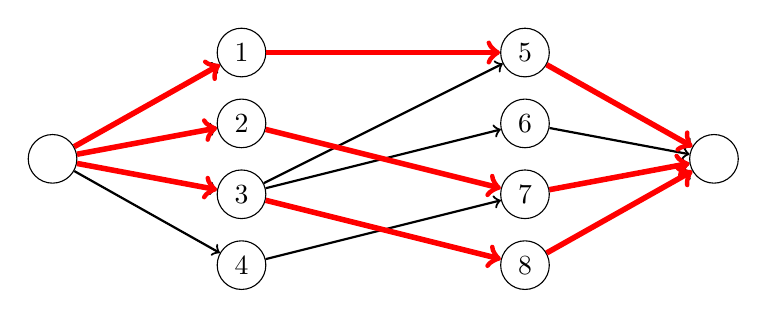
\begin{tikzpicture}[scale=0.60]
	\node[draw, circle] (1) at (2,4.5) {1};
	\node[draw, circle] (2) at (2,3) {2};
	\node[draw, circle] (3) at (2,1.5) {3};
	\node[draw, circle] (4) at (2,0) {4};
	\node[draw, circle] (5) at (8,4.5) {5};
	\node[draw, circle] (6) at (8,3) {6};
	\node[draw, circle] (7) at (8,1.5) {7};
	\node[draw, circle] (8) at (8,0) {8};

	\node[draw, circle] (a) at (-2,2.25) {\phantom{0}};
	\node[draw, circle] (b) at (12,2.25) {\phantom{0}};

	%\path[draw,thick,->] (1) -- (5);
	%\path[draw,thick,->] (2) -- (7);
	\path[draw,thick,->] (3) -- (5);
	\path[draw,thick,->] (3) -- (6);
	%\path[draw,thick,->] (3) -- (8);
	\path[draw,thick,->] (4) -- (7);

	\path[draw,thick,->] (a) -- (1);
	\path[draw,thick,->] (a) -- (2);
	\path[draw,thick,->] (a) -- (3);
	\path[draw,thick,->] (a) -- (4);
	\path[draw,thick,->] (5) -- (b);
	\path[draw,thick,->] (6) -- (b);
	\path[draw,thick,->] (7) -- (b);
	\path[draw,thick,->] (8) -- (b);

	\path[draw=red,thick,->,line width=2pt] (1) -- (5);
	\path[draw=red,thick,->,line width=2pt] (2) -- (7);
	\path[draw=red,thick,->,line width=2pt] (3) -- (8);

	\path[draw=red,thick,->,line width=2pt] (a) -- (1);
	\path[draw=red,thick,->,line width=2pt] (a) -- (2);
	\path[draw=red,thick,->,line width=2pt] (a) -- (3);

	\path[draw=red,thick,->,line width=2pt] (5) -- (b);
	\path[draw=red,thick,->,line width=2pt] (7) -- (b);
	\path[draw=red,thick,->,line width=2pt] (8) -- (b);

	\end{tikzpicture}
\end{center}

\subsubsection{Teorema de Hall}

\index{teorema de Hall}
\index{emparejamiento perfecto}

El \key{teorema de Hall} se puede utilizar para saber
si un grafo bipartito tiene un emparejamiento que contenga a
todos los nodos de la izquierda o de la derecha.
Si la cantidad de nodos en la izquierda y en la derecha es la misma,
el teorema de Hall nos dice si es posible
construir un \key{emparejamiento perfecto} que
contenga todos los nodos del grafo.

Asuma que queremos encontrar un emparejamiento
que contenga todos los nodos de la izquierda.
Sea $X$ cualquier conjunto de nodos de la izquierda
y sea $f(X)$ el conjunto de sus vecinos.
De acuerdo al teorema de Hall, existe un emparejamiento
que contiene a todos los nodos de la izquierda
exactamente cuando para cada $X$, se cumple la condici\'on $|X| \le |f(X)|$.

Estudiemos el teorema de Hall en el grafo de ejemplo.
Primero, sea $X=\{1,3\}$ y $f(X)=\{5,6,8\}$:

\begin{center}
	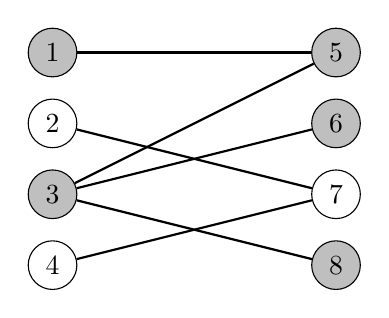
\begin{tikzpicture}[scale=0.60]
	\node[draw, circle, fill=lightgray] (1) at (2,4.5) {1};
	\node[draw, circle] (2) at (2,3) {2};
	\node[draw, circle, fill=lightgray] (3) at (2,1.5) {3};
	\node[draw, circle] (4) at (2,0) {4};
	\node[draw, circle, fill=lightgray] (5) at (8,4.5) {5};
	\node[draw, circle, fill=lightgray] (6) at (8,3) {6};
	\node[draw, circle] (7) at (8,1.5) {7};
	\node[draw, circle, fill=lightgray] (8) at (8,0) {8};

	\path[draw,thick,-] (1) -- (5);
	\path[draw,thick,-] (2) -- (7);
	\path[draw,thick,-] (3) -- (5);
	\path[draw,thick,-] (3) -- (6);
	\path[draw,thick,-] (3) -- (8);
	\path[draw,thick,-] (4) -- (7);
	\end{tikzpicture}
\end{center}

La condici\'on del teorema de Hall se cumple, ya que
$|X|=2$ y $|f(X)|=3$.
En el siguiente ejemplo, sean $X=\{2,4\}$ y $f(X)=\{7\}$:

\begin{center}
	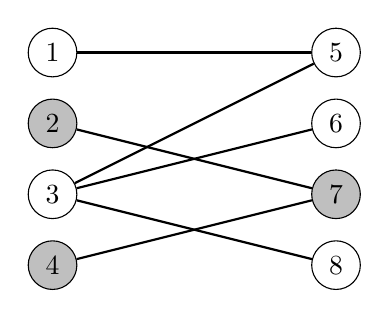
\begin{tikzpicture}[scale=0.60]
	\node[draw, circle] (1) at (2,4.5) {1};
	\node[draw, circle, fill=lightgray] (2) at (2,3) {2};
	\node[draw, circle] (3) at (2,1.5) {3};
	\node[draw, circle, fill=lightgray] (4) at (2,0) {4};
	\node[draw, circle] (5) at (8,4.5) {5};
	\node[draw, circle] (6) at (8,3) {6};
	\node[draw, circle, fill=lightgray] (7) at (8,1.5) {7};
	\node[draw, circle] (8) at (8,0) {8};

	\path[draw,thick,-] (1) -- (5);
	\path[draw,thick,-] (2) -- (7);
	\path[draw,thick,-] (3) -- (5);
	\path[draw,thick,-] (3) -- (6);
	\path[draw,thick,-] (3) -- (8);
	\path[draw,thick,-] (4) -- (7);
	\end{tikzpicture}
\end{center}

En este caso, $|X|=2$ y $|f(X)|=1$,
por lo tanto no se cumple la condici\'on de Hall.
Lo que significa que no es posible formar
un emparejamiento perfecto en el grafo.
Este resultado no sorprende, debido a que ya
sabemos que el emparejamiento m\'aximo del grafo es 3 y no 4.

Si la condici\'on del teorema de Hall no se cumple,
el conjunto $X$ provee una explicaci\'on del \emph{por qu\'e}
no podemos formar tal emparejamiento.
Dado que $X$ contiene m\'as nodos que $f(X)$,
no existe una pareja de nodos para todos los nodos en $X$.
Por ejemplo, en el grafo anterior, ambos nodos 2 y 4
deben conectarse con el nodo 7, lo que no est\'a permitido.

\subsubsection{Teorema de Kőnig}

\index{teorema de Kőnig}
\index{cubierta de nodos}
\index{cubierta m\'inima de nodos}

Una \key{cubierta m\'inima de nodos} de un grafo
es un conjunto m\'inimo de nodos tal que cada arista del grafo
tiene al menos uno de sus nodos en el conjunto.
En un grafo general, encontrar la cubierta m\'inima de nodos
es un problema NP duro.
Sin embargo, si el grafo es bipartito,
el \key{terorema de Kőnig} nos dice que
el tama\~no de la cubierta m\'inima de nodos
y el tama\~no del emparejamiento m\'aximo siempre son iguales.
Por lo que podemos calcular el tama\~no de la cubierta m\'inima de nodos
utilizando un algoritmo de flujo m\'aximo.

Tomemos en consideraci\'on el siguiente grafo
con un emparejamiento m\'aximo de tama\~no 3:
\begin{center}
	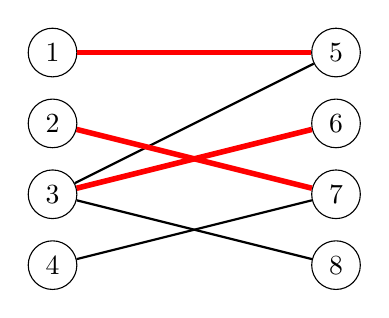
\begin{tikzpicture}[scale=0.60]
	\node[draw, circle] (1) at (2,4.5) {1};
	\node[draw, circle] (2) at (2,3) {2};
	\node[draw, circle] (3) at (2,1.5) {3};
	\node[draw, circle] (4) at (2,0) {4};
	\node[draw, circle] (5) at (8,4.5) {5};
	\node[draw, circle] (6) at (8,3) {6};
	\node[draw, circle] (7) at (8,1.5) {7};
	\node[draw, circle] (8) at (8,0) {8};

	\path[draw,thick,-] (1) -- (5);
	\path[draw,thick,-] (2) -- (7);
	\path[draw,thick,-] (3) -- (5);
	\path[draw,thick,-] (3) -- (6);
	\path[draw,thick,-] (3) -- (8);
	\path[draw,thick,-] (4) -- (7);

	\path[draw=red,thick,-,line width=2pt] (1) -- (5);
	\path[draw=red,thick,-,line width=2pt] (2) -- (7);
	\path[draw=red,thick,-,line width=2pt] (3) -- (6);
	\end{tikzpicture}
\end{center}
El teorema de Kőnig plantea que el tama\~no
de una cubierta m\'inima de nodos tambi\'en es 3.
Se puede construir de la siguiente manera:

\begin{center}
	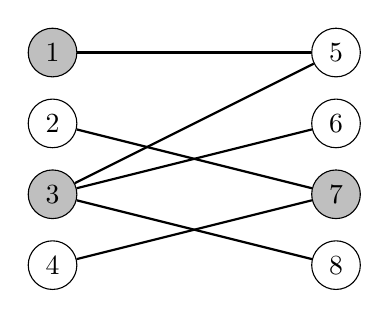
\begin{tikzpicture}[scale=0.60]
	\node[draw, circle, fill=lightgray] (1) at (2,4.5) {1};
	\node[draw, circle] (2) at (2,3) {2};
	\node[draw, circle, fill=lightgray] (3) at (2,1.5) {3};
	\node[draw, circle] (4) at (2,0) {4};
	\node[draw, circle] (5) at (8,4.5) {5};
	\node[draw, circle] (6) at (8,3) {6};
	\node[draw, circle, fill=lightgray] (7) at (8,1.5) {7};
	\node[draw, circle] (8) at (8,0) {8};

	\path[draw,thick,-] (1) -- (5);
	\path[draw,thick,-] (2) -- (7);
	\path[draw,thick,-] (3) -- (5);
	\path[draw,thick,-] (3) -- (6);
	\path[draw,thick,-] (3) -- (8);
	\path[draw,thick,-] (4) -- (7);
	\end{tikzpicture}
\end{center}

\index{conjunto independiente}
\index{conjunto independiente m\'aximo}

Los nodos que \emph{no}
pertenecen a una cubierta m\'inima de nodos
forman un \key{conjunto independiente m\'aximo}.
Este es el mayor cojunto posible de nodos
donde no existen dos nodos
conectados por una arista.
Una vez m\'as, encontrar un conjunto independiente m\'aximo
en un grafo general es un problema NP duro,
pero en un grafo bipartito se puede utilizar
el teorema de Kőnig para resolver el problema de manera eficiente.
En el grafo de ejemplo, el conjunto independiente m\'aximo
es el que se muestra a continuaci\'on:

\begin{center}
	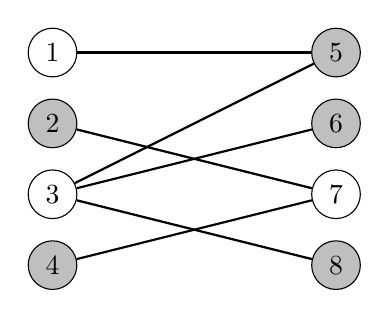
\begin{tikzpicture}[scale=0.60]
	\node[draw, circle] (1) at (2,4.5) {1};
	\node[draw, circle, fill=lightgray] (2) at (2,3) {2};
	\node[draw, circle] (3) at (2,1.5) {3};
	\node[draw, circle, fill=lightgray] (4) at (2,0) {4};
	\node[draw, circle, fill=lightgray] (5) at (8,4.5) {5};
	\node[draw, circle, fill=lightgray] (6) at (8,3) {6};
	\node[draw, circle] (7) at (8,1.5) {7};
	\node[draw, circle, fill=lightgray] (8) at (8,0) {8};

	\path[draw,thick,-] (1) -- (5);
	\path[draw,thick,-] (2) -- (7);
	\path[draw,thick,-] (3) -- (5);
	\path[draw,thick,-] (3) -- (6);
	\path[draw,thick,-] (3) -- (8);
	\path[draw,thick,-] (4) -- (7);
	\end{tikzpicture}
\end{center}

\section{Cubierta de caminos}

\index{cubierta de caminos}

Una \key{cubierta de caminos} es un conjunto de caminos en un grafo
donde cada nodo del grafo pertenece a uno de los caminos.
Resulta que en un grafo dirigido ac\'iclico
se puede reducir el problema de encontrar una cubierta de caminos m\'inima
al problema de encontrar el flujo
m\'aximo en otro grafo.

\subsubsection{Cubierta de caminos disjunta en los nodos}

En una \key{cubierta de caminos disjunta en los nodos},
cada nodo pertenece exactamente a un camino.
Como ejemplo, considera el siguiente grafo:
\begin{center}
	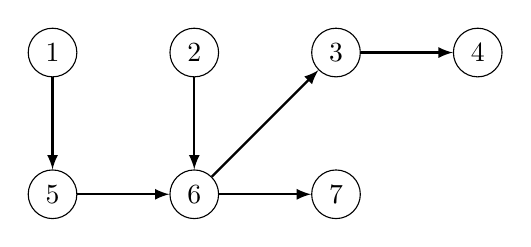
\begin{tikzpicture}[scale=0.9]
	\node[draw, circle] (1) at (0,0) {1};
	\node[draw, circle] (2) at (2,0) {2};
	\node[draw, circle] (3) at (4,0) {3};
	\node[draw, circle] (4) at (6,0) {4};
	\node[draw, circle] (5) at (0,-2) {5};
	\node[draw, circle] (6) at (2,-2) {6};
	\node[draw, circle] (7) at (4,-2) {7};

	\path[draw,thick,->,>=latex] (1) -- (5);
	\path[draw,thick,->,>=latex] (2) -- (6);
	\path[draw,thick,->,>=latex] (3) -- (4);
	\path[draw,thick,->,>=latex] (5) -- (6);
	\path[draw,thick,->,>=latex] (6) -- (3);
	\path[draw,thick,->,>=latex] (6) -- (7);
	\end{tikzpicture}
\end{center}

Una cubierta de caminos disjunta en los nodos m\'inima
de este grafo
consiste de tres caminos.
Por ejemplo, podemos seleccionar los siguientes caminos:

\begin{center}
	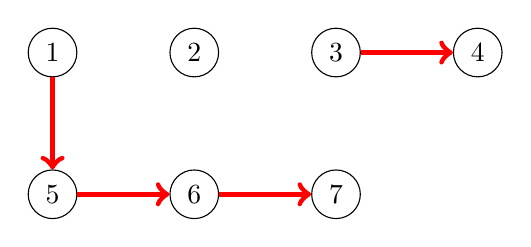
\begin{tikzpicture}[scale=0.9]
	\node[draw, circle] (1) at (0,0) {1};
	\node[draw, circle] (2) at (2,0) {2};
	\node[draw, circle] (3) at (4,0) {3};
	\node[draw, circle] (4) at (6,0) {4};
	\node[draw, circle] (5) at (0,-2) {5};
	\node[draw, circle] (6) at (2,-2) {6};
	\node[draw, circle] (7) at (4,-2) {7};

	\path[draw=red,thick,->,line width=2pt] (1) -- (5);
	\path[draw=red,thick,->,line width=2pt] (5) -- (6);
	\path[draw=red,thick,->,line width=2pt] (6) -- (7);
	\path[draw=red,thick,->,line width=2pt] (3) -- (4);
	\end{tikzpicture}
\end{center}

Tenga en cuenta que uno de los caminos solamente contiene al nodo 2,
por lo que es posible que un camino no contenga a ninguna arista.

Podemos encontrar una cubierta de caminos disjunta en los nodos
construyendo un grafo de emparejamiento donde cada nodo
del grafo original se representa con
dos nodos: un nodo izquierdo y uno derecho.
Existe una arista desde el nodo izquierdo hacia el nodo derecho
siempre que la arista tambi\'en exista en el grafo original.
Adem\'as, el grafo de emparejamiento contiene una fuente y un sumidero
donde existen aristas desde la fuente hacia todos los
nodos izquierdos y desde todos los nodos derechos hacia el sumidero.

Un emparejamiento m\'aximo en el grafo resultante corresponde
a la cubierta de caminos disjunta en los nodos m\'inima en
el grafo original.
Por ejemplo, el siguiente grafo contiene
un emparejamiento m\'aximo de tama\~no 4:

\begin{center}
	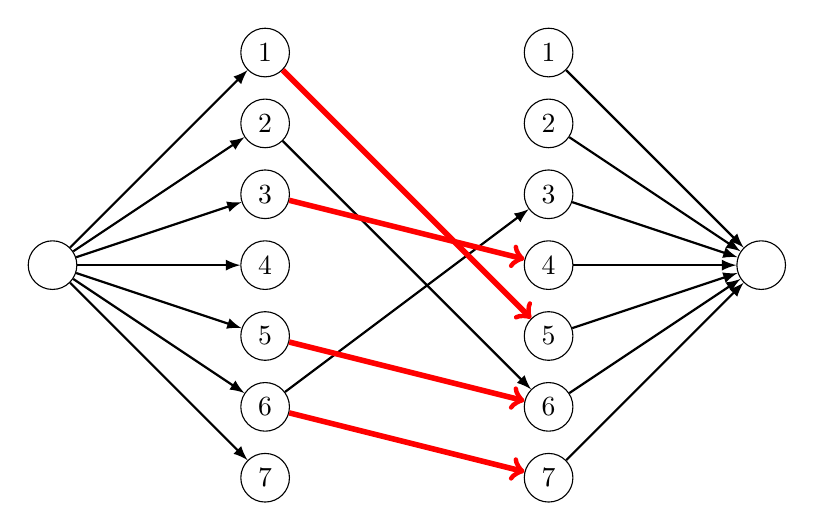
\begin{tikzpicture}[scale=0.9]
	\node[draw, circle] (1a) at (0,6) {1};
	\node[draw, circle] (2a) at (0,5) {2};
	\node[draw, circle] (3a) at (0,4) {3};
	\node[draw, circle] (4a) at (0,3) {4};
	\node[draw, circle] (5a) at (0,2) {5};
	\node[draw, circle] (6a) at (0,1) {6};
	\node[draw, circle] (7a) at (0,0) {7};

	\node[draw, circle] (1b) at (4,6) {1};
	\node[draw, circle] (2b) at (4,5) {2};
	\node[draw, circle] (3b) at (4,4) {3};
	\node[draw, circle] (4b) at (4,3) {4};
	\node[draw, circle] (5b) at (4,2) {5};
	\node[draw, circle] (6b) at (4,1) {6};
	\node[draw, circle] (7b) at (4,0) {7};

	\node[draw, circle] (a) at (-3,3) {\phantom{0}};
	\node[draw, circle] (b) at (7,3) {\phantom{0}};

	%\path[draw,thick,->,>=latex] (1a) -- (5b);
	\path[draw,thick,->,>=latex] (2a) -- (6b);
	%\path[draw,thick,->,>=latex] (3a) -- (4b);
	%\path[draw,thick,->,>=latex] (5a) -- (6b);
	\path[draw,thick,->,>=latex] (6a) -- (3b);
	%\path[draw,thick,->,>=latex] (6a) -- (7b);

	\path[draw,thick,->,>=latex] (a) -- (1a);
	\path[draw,thick,->,>=latex] (a) -- (2a);
	\path[draw,thick,->,>=latex] (a) -- (3a);
	\path[draw,thick,->,>=latex] (a) -- (4a);
	\path[draw,thick,->,>=latex] (a) -- (5a);
	\path[draw,thick,->,>=latex] (a) -- (6a);
	\path[draw,thick,->,>=latex] (a) -- (7a);

	\path[draw,thick,->,>=latex] (1b) -- (b);
	\path[draw,thick,->,>=latex] (2b) -- (b);
	\path[draw,thick,->,>=latex] (3b) -- (b);
	\path[draw,thick,->,>=latex] (4b) -- (b);
	\path[draw,thick,->,>=latex] (5b) -- (b);
	\path[draw,thick,->,>=latex] (6b) -- (b);
	\path[draw,thick,->,>=latex] (7b) -- (b);

	\path[draw=red,thick,->,line width=2pt] (1a) -- (5b);
	\path[draw=red,thick,->,line width=2pt] (5a) -- (6b);
	\path[draw=red,thick,->,line width=2pt] (6a) -- (7b);
	\path[draw=red,thick,->,line width=2pt] (3a) -- (4b);

	\end{tikzpicture}
\end{center}

Cada arista en el emparejamiento m\'aximo del grafo de emparejamiento corresponde
a una arista en la cubierta de caminos disjunta en los nodos m\'inima del
grafo original.
Por lo tanto, el tama\~no de la cubierta de caminos disjunta en los nodos m\'inima es $n-c$,
donde $n$ es la cantidad de nodos en el grafo original
y $c$ es el tama\~no del emparejamiento m\'aximo.

\subsubsection{Cubierta general de caminos}

Una \key{cubierta general de caminos} es una cubierta de caminos
donde un nodo puede pertenecer a m\'as de un camino.
Una cubierta general de caminos m\'inima puede ser menor
que una cubierta de caminos disjunta en los nodos m\'inima,
ya que un nodo puede ser utilizado varias veces en los caminos.
Considere nuevamente el siguiente grafo:
\begin{center}
	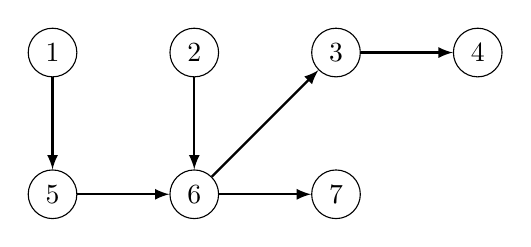
\begin{tikzpicture}[scale=0.9]
	\node[draw, circle] (1) at (0,0) {1};
	\node[draw, circle] (2) at (2,0) {2};
	\node[draw, circle] (3) at (4,0) {3};
	\node[draw, circle] (4) at (6,0) {4};
	\node[draw, circle] (5) at (0,-2) {5};
	\node[draw, circle] (6) at (2,-2) {6};
	\node[draw, circle] (7) at (4,-2) {7};

	\path[draw,thick,->,>=latex] (1) -- (5);
	\path[draw,thick,->,>=latex] (2) -- (6);
	\path[draw,thick,->,>=latex] (3) -- (4);
	\path[draw,thick,->,>=latex] (5) -- (6);
	\path[draw,thick,->,>=latex] (6) -- (3);
	\path[draw,thick,->,>=latex] (6) -- (7);
	\end{tikzpicture}
\end{center}

La cubierta general de caminos en este grafo
consiste de dos caminos.
Por ejemplo, el primer camino puede ser como se muestra a continuaci\'on:
\begin{center}
	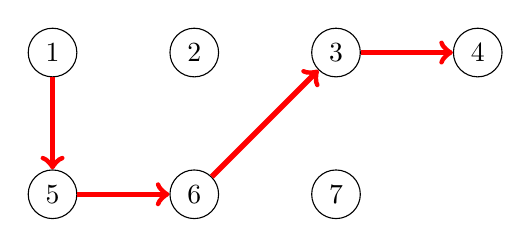
\begin{tikzpicture}[scale=0.9]
	\node[draw, circle] (1) at (0,0) {1};
	\node[draw, circle] (2) at (2,0) {2};
	\node[draw, circle] (3) at (4,0) {3};
	\node[draw, circle] (4) at (6,0) {4};
	\node[draw, circle] (5) at (0,-2) {5};
	\node[draw, circle] (6) at (2,-2) {6};
	\node[draw, circle] (7) at (4,-2) {7};

	\path[draw=red,thick,->,line width=2pt] (1) -- (5);
	\path[draw=red,thick,->,line width=2pt] (5) -- (6);
	\path[draw=red,thick,->,line width=2pt] (6) -- (3);
	\path[draw=red,thick,->,line width=2pt] (3) -- (4);
	\end{tikzpicture}
\end{center}
Y el segundo camino como se muestra a continuaci\'on:
\begin{center}
	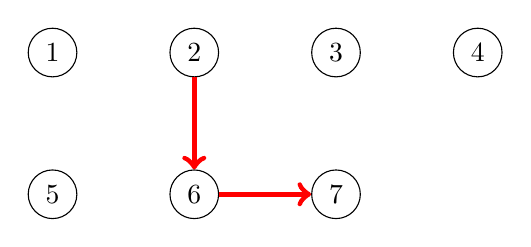
\begin{tikzpicture}[scale=0.9]
	\node[draw, circle] (1) at (0,0) {1};
	\node[draw, circle] (2) at (2,0) {2};
	\node[draw, circle] (3) at (4,0) {3};
	\node[draw, circle] (4) at (6,0) {4};
	\node[draw, circle] (5) at (0,-2) {5};
	\node[draw, circle] (6) at (2,-2) {6};
	\node[draw, circle] (7) at (4,-2) {7};

	\path[draw=red,thick,->,line width=2pt] (2) -- (6);
	\path[draw=red,thick,->,line width=2pt] (6) -- (7);
	\end{tikzpicture}
\end{center}

Una cubierta general de caminos m\'inima se puede encontrar
casi de la misma manera que una cubierta de caminos disjunta en los nodos.
Solo basta con agregar algunas aristas nuevas al grafo de emparejamiento
de tal forma que exista una arista $a \rightarrow b$
siempre que exista un camino desde $a$ hacia $b$
en el grafo original (posiblemente pasando por varias aristas).

A continuaci\'on, se muestra el grafo de emparejamiento para el grafo anterior:
\begin{center}
	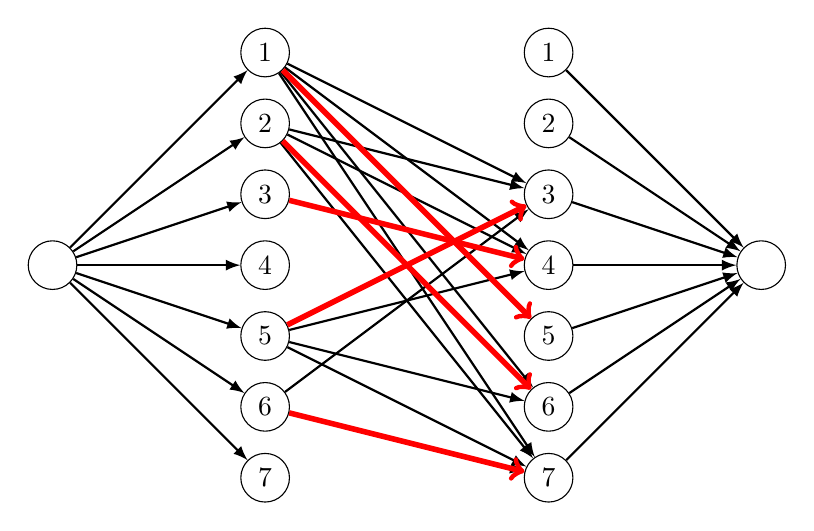
\begin{tikzpicture}[scale=0.9]
	\node[draw, circle] (1a) at (0,6) {1};
	\node[draw, circle] (2a) at (0,5) {2};
	\node[draw, circle] (3a) at (0,4) {3};
	\node[draw, circle] (4a) at (0,3) {4};
	\node[draw, circle] (5a) at (0,2) {5};
	\node[draw, circle] (6a) at (0,1) {6};
	\node[draw, circle] (7a) at (0,0) {7};

	\node[draw, circle] (1b) at (4,6) {1};
	\node[draw, circle] (2b) at (4,5) {2};
	\node[draw, circle] (3b) at (4,4) {3};
	\node[draw, circle] (4b) at (4,3) {4};
	\node[draw, circle] (5b) at (4,2) {5};
	\node[draw, circle] (6b) at (4,1) {6};
	\node[draw, circle] (7b) at (4,0) {7};

	\node[draw, circle] (a) at (-3,3) {\phantom{0}};
	\node[draw, circle] (b) at (7,3) {\phantom{0}};


	%\path[draw,thick,->,>=latex] (1a) -- (5b);
	\path[draw,thick,->,>=latex] (1a) -- (6b);
	\path[draw,thick,->,>=latex] (1a) -- (7b);
	\path[draw,thick,->,>=latex] (1a) -- (3b);
	\path[draw,thick,->,>=latex] (1a) -- (4b);
	\path[draw,thick,->,>=latex] (5a) -- (6b);
	\path[draw,thick,->,>=latex] (5a) -- (7b);
	%\path[draw,thick,->,>=latex] (5a) -- (3b);
	\path[draw,thick,->,>=latex] (5a) -- (4b);
	\path[draw,thick,->,>=latex] (6a) -- (7b);
	%\path[draw,thick,->,>=latex] (6a) -- (7b);
	\path[draw,thick,->,>=latex] (6a) -- (3b);
	%\path[draw,thick,->,>=latex] (3a) -- (4b);
	%\path[draw,thick,->,>=latex] (2a) -- (6b);
	\path[draw,thick,->,>=latex] (2a) -- (7b);
	\path[draw,thick,->,>=latex] (2a) -- (3b);
	\path[draw,thick,->,>=latex] (2a) -- (4b);


	\path[draw,thick,->,>=latex] (a) -- (1a);
	\path[draw,thick,->,>=latex] (a) -- (2a);
	\path[draw,thick,->,>=latex] (a) -- (3a);
	\path[draw,thick,->,>=latex] (a) -- (4a);
	\path[draw,thick,->,>=latex] (a) -- (5a);
	\path[draw,thick,->,>=latex] (a) -- (6a);
	\path[draw,thick,->,>=latex] (a) -- (7a);

	\path[draw,thick,->,>=latex] (1b) -- (b);
	\path[draw,thick,->,>=latex] (2b) -- (b);
	\path[draw,thick,->,>=latex] (3b) -- (b);
	\path[draw,thick,->,>=latex] (4b) -- (b);
	\path[draw,thick,->,>=latex] (5b) -- (b);
	\path[draw,thick,->,>=latex] (6b) -- (b);
	\path[draw,thick,->,>=latex] (7b) -- (b);

	\path[draw=red,thick,->,line width=2pt] (1a) -- (5b);
	\path[draw=red,thick,->,line width=2pt] (5a) -- (3b);
	\path[draw=red,thick,->,line width=2pt] (3a) -- (4b);
	\path[draw=red,thick,->,line width=2pt] (2a) -- (6b);
	\path[draw=red,thick,->,line width=2pt] (6a) -- (7b);


	% \path[draw=red,thick,->,line width=2pt] (1a) -- (6b);
	% \path[draw=red,thick,->,line width=2pt] (1a) -- (7b);
	% \path[draw=red,thick,->,line width=2pt] (1a) -- (3b);
	% \path[draw=red,thick,->,line width=2pt] (1a) -- (4b);
	% \path[draw=red,thick,->,line width=2pt] (5a) -- (6b);
	% \path[draw=red,thick,->,line width=2pt] (5a) -- (7b);
	% \path[draw=red,thick,->,line width=2pt] (5a) -- (3b);
	% \path[draw=red,thick,->,line width=2pt] (5a) -- (4b);
	% \path[draw=red,thick,->,line width=2pt] (6a) -- (7b);
	% \path[draw=red,thick,->,line width=2pt] (6a) -- (7b);
	% \path[draw=red,thick,->,line width=2pt] (6a) -- (3b);
	% \path[draw=red,thick,->,line width=2pt] (3a) -- (4b);
	% \path[draw=red,thick,->,line width=2pt] (2a) -- (6b);
	% \path[draw=red,thick,->,line width=2pt] (2a) -- (7b);
	% \path[draw=red,thick,->,line width=2pt] (2a) -- (3b);
	% \path[draw=red,thick,->,line width=2pt] (2a) -- (4b);

	\end{tikzpicture}
\end{center}

\subsubsection{Teorema de Dilworth}

\index{teorema de Dilworth}
\index{anticadena}

Una \key{anticadena} es un conjunto de nodos de un grafo
donde existe un camino
desde cualquier nodo hacia cualquier otro nodo
utilizando las aristas del grafo.
El \key{teorema de Dilworth} plantea que
en un grafo dirigido ac\'iclico, el tama\~no
de una cubierta general de caminos m\'inima
es igual al tama\~no de una anticadena m\'axima.

Por ejemplo, los nodos 3 y 7 forman una anticadena
en el siguiente grafo:

\begin{center}
	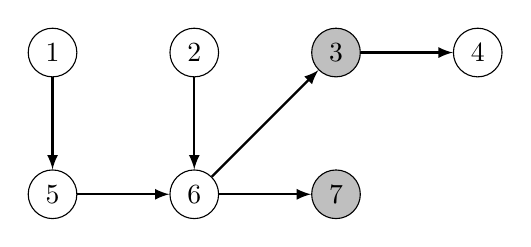
\begin{tikzpicture}[scale=0.9]
	\node[draw, circle] (1) at (0,0) {1};
	\node[draw, circle] (2) at (2,0) {2};
	\node[draw, circle, fill=lightgray] (3) at (4,0) {3};
	\node[draw, circle] (4) at (6,0) {4};
	\node[draw, circle] (5) at (0,-2) {5};
	\node[draw, circle] (6) at (2,-2) {6};
	\node[draw, circle, fill=lightgray] (7) at (4,-2) {7};

	\path[draw,thick,->,>=latex] (1) -- (5);
	\path[draw,thick,->,>=latex] (2) -- (6);
	\path[draw,thick,->,>=latex] (3) -- (4);
	\path[draw,thick,->,>=latex] (5) -- (6);
	\path[draw,thick,->,>=latex] (6) -- (3);
	\path[draw,thick,->,>=latex] (6) -- (7);
	\end{tikzpicture}
\end{center}

Este conjunto representa una anticadena m\'axima, ya que no es posible
construir ninguna anticadena que pueda contener tres nodos.
Hemos visto anteriormente que el tama\~no de una cubierta
general de caminos m\'inima de este grafo consiste de dos caminos.
